\documentclass[11pt]{article}
\usepackage[margin=0.7in, top=0.5in]{geometry}
\usepackage[all]{nowidow}
\usepackage[hyperfigures=true, hidelinks, pdfhighlight=/N]{hyperref}
\usepackage[separate-uncertainty=true, group-digits=false]{siunitx}
\usepackage{graphicx,amsmath,physics,tabto,float,amssymb,pgfplots,verbatim,tcolorbox}
\usepackage{listings,xcolor,subfig,caption,import,wrapfig,biblatex}
\usepackage[version=4]{mhchem}
\usepackage[noabbrev]{cleveref}
\newcommand{\creflastconjunction}{, and\nobreakspace}
\newcommand{\mb}[1]{\mathbf{#1}}
\newcommand{\chisq}{\chi^2}
\newcommand{\chisqdof}{\chi^2/\mathrm{dof}}
\numberwithin{equation}{section}
\numberwithin{figure}{section}
\numberwithin{table}{section}
\definecolor{stringcolor}{HTML}{C792EA}
\definecolor{codeblue}{HTML}{2162DB}
\definecolor{commentcolor}{HTML}{4A6E46}
\captionsetup{font=small, belowskip=0pt}
\lstdefinestyle{appendix}{
    basicstyle=\ttfamily\footnotesize,commentstyle=\color{commentcolor},keywordstyle=\color{codeblue},
    stringstyle=\color{stringcolor},showstringspaces=false,numbers=left,upquote=true,captionpos=t,
    abovecaptionskip=12pt,belowcaptionskip=12pt,language=Python,breaklines=true,frame=single}
\lstdefinestyle{inline}{
    basicstyle=\ttfamily\footnotesize,commentstyle=\color{commentcolor},keywordstyle=\color{codeblue},
    stringstyle=\color{stringcolor},showstringspaces=false,numbers=left,upquote=true,frame=tb,
    captionpos=b,language=Python}
\renewcommand{\lstlistingname}{Appendix}
\pgfplotsset{compat=1.17}
\addbibresource{bibliography.bib}

\begin{document}

\begin{center}
    {\huge How Much Higgs?}\\
    \vspace{0.2in}
    \textbf{KDSMIL001 | September 2022}
    
    
\end{center}

\section{Introduction}\label{sec:Introduction}
This report aims to investigate the $\chi^2$ and p-value test statistics using data from the ATLAS experiment, reconstructing the mass of the Higgs boson from the 4-lepton system. Our model gives us predictions for the background signal as well as the signal around the Higgs mass. To fit this model to our data we use two parameters: $s_s$ multiplying the Higgs signal and $s_b$ multiplying the background. 

Fitting just one of these parameters at a time, we can have a first look at the $\chi^2$ statistic. This 

, and then try out a two-parameter fit. Using this fit, we can

Two single-parameter fits of our model to the data are performed

\section{Exercises}\label{sec:Exercises}
Before fitting our model to the data, we first looked at the quality of the fit as it came from the data provided. \Cref{fig:no_fit_hist} shows the data, with $\chisq/\mathrm{dof}=\num{1.598}$. This is a reasonable value as it's close to 1, but we can definitely do better. 

\begin{figure}[h]
    \begin{center}
        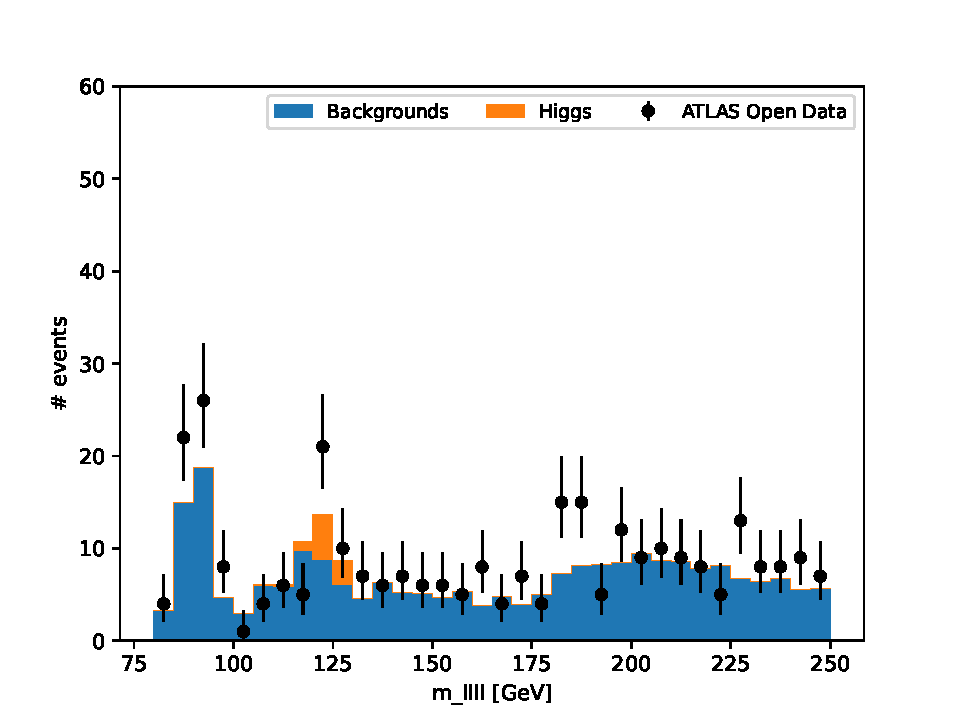
\includegraphics[width=.6\textwidth]{Plots/no_fit_hist.pdf}
        \caption{ATLAS open data of the mass of the 4-lepton system around the predicted mass of the Higgs boson. Also shown is the simulated prediction for the distribution of masses, made up of a background signal and a Higgs signal. For this model, $\chisqdof=\num{1.598}$.}
        \label{fig:no_fit_hist}
    \end{center}
\end{figure}

Our first attempts at fitting the model to our data were one-parameter fits, changing the multiplicative factor $s_s$ for the Higgs signal first. At each new value we found a $\chisq$ value for the fit then subtracted the lowest value from the entire set, giving us a $\Delta\chisq$ value for each $s_s$ value in our interval. For a one-parameter fit, a confidence interval of $68\%$ is defined as all values for which $\Delta\chisq\leq1$~\cite{XRay_energy_spectra}. From this we could extract an uncertainty on the best-fit parameter. Our best-fit value was found to be $s_s=\num{2.01 \pm0.76}$ with $\chisqdof=1.558$.

Doing the same but for $s_b$, multiplying the background signal, we found $s_b=\num{1.302\pm0.076}$ with $\chisqdof=1.018$. This parameter clearly has more of an impact on the fit than $s_s$ as can be seen from the lower $\chisqdof$ value. It also has a smaller uncertainty, which is interesting. \textbf{\textit{SOME REASONING HERE}}

Of course, fitting just one parameter at a time is naive, so we then fit them both at the same time, looping over both and finding the minimum $\chisq$ point. This gave us best-fit values of $s_s=1.39^{+1.16}_{-0.87}$ and $s_b=1.29^{+0.12}_{-0.11}$. The estimation of these uncertainties came again from the $68\%$ confidence interval, defined for a two-parameter fit as all pairs of values for which $\Delta\chisq\leq2.3$~\cite{XRay_energy_spectra}. This critical value, as it's called, of 2.3 will be investigated later on. This two-parameter fit had $\chisqdof=1.039$.

\begin{figure}[h]
    \begin{center}
        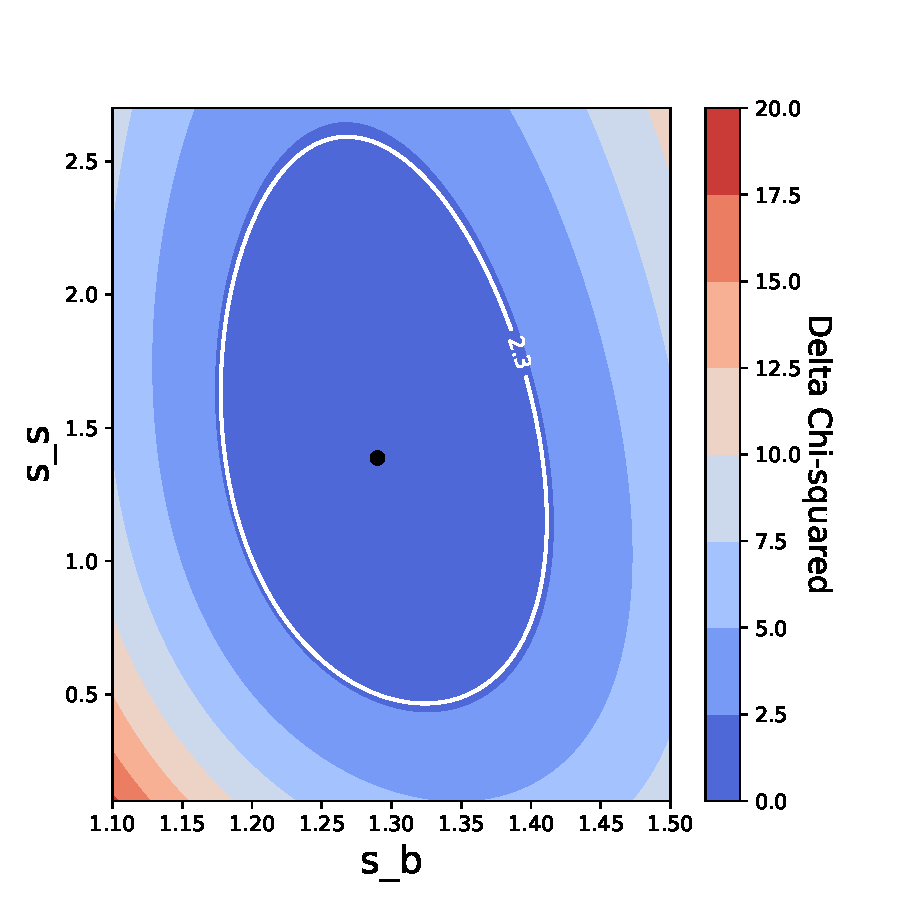
\includegraphics[width=.6\textwidth]{Plots/two_fit_contour.pdf}
        \caption{Contour plot showing the $\Delta\chisq$ value for each $(s_s,\,s_b)$ pair. The confidence interval on the best-fit pair is shown as the area inside the contour at $\Delta\chisq=2.3$. Upper and lower bounds on the confidence interval for each parameter were extracted to determine uncertainties. $chisqdof=1.039$.}
        \label{fig:two_fit_contour}
    \end{center}
\end{figure}





\newpage
\printbibliography

\end{document}